\section{Evaluation}
We evaluated the success of the software engineering on this project by performing the same quantitative analyses on the codebase and analysing the performance gains of the new analysis algorithms.

\begin{figure}[ptb]
\begin{center}
\subcaptionbox{The original PIPE 4 tangle graph reporting four tangles of size 18, 10, 7 and 5.}{
    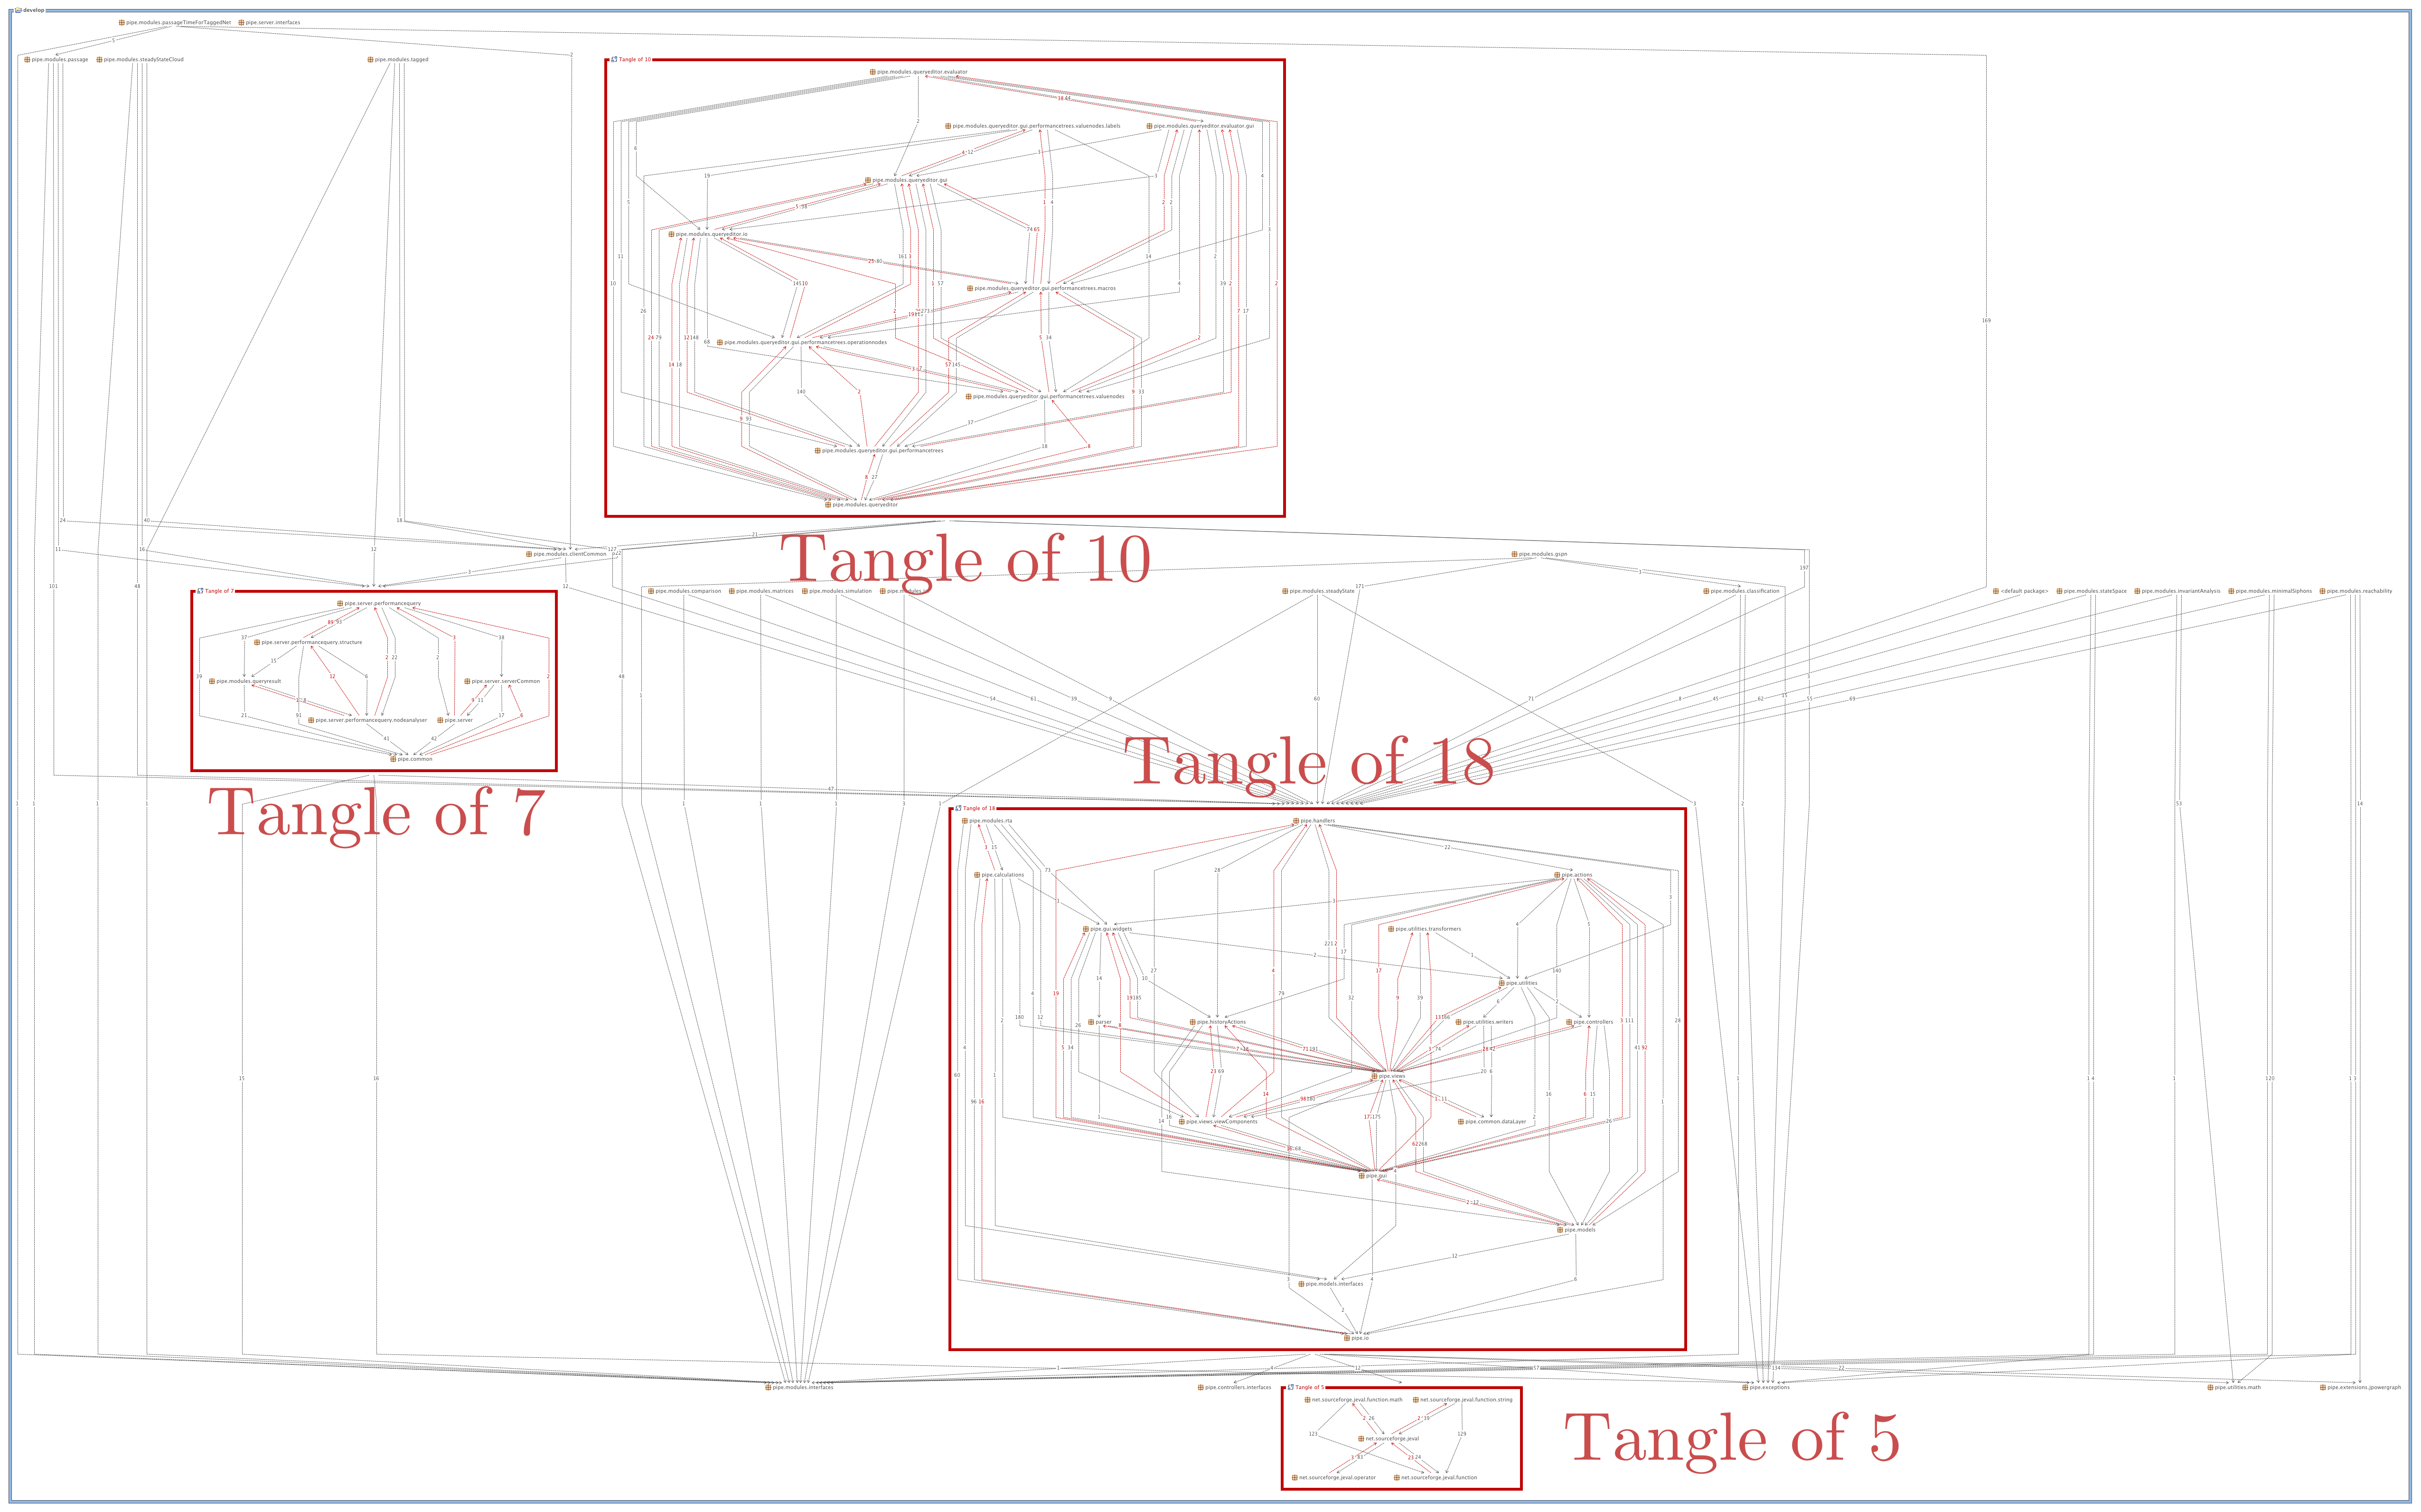
\includegraphics[width=0.85\textwidth]{eval/original_tangle_annotated.png} 
}
\subcaptionbox{The tangle graph for the PIPE repository housing the view code in PIPE 5 which contains the Swing GUI code. It contains only a single tangle of size 11. Unfortunately due to time constraints PIPE 5 uses much of the original PIPE 4 architecture which is why we were not able to reduce the tangle count further as many of the existing classes are tightly coupled. }{
    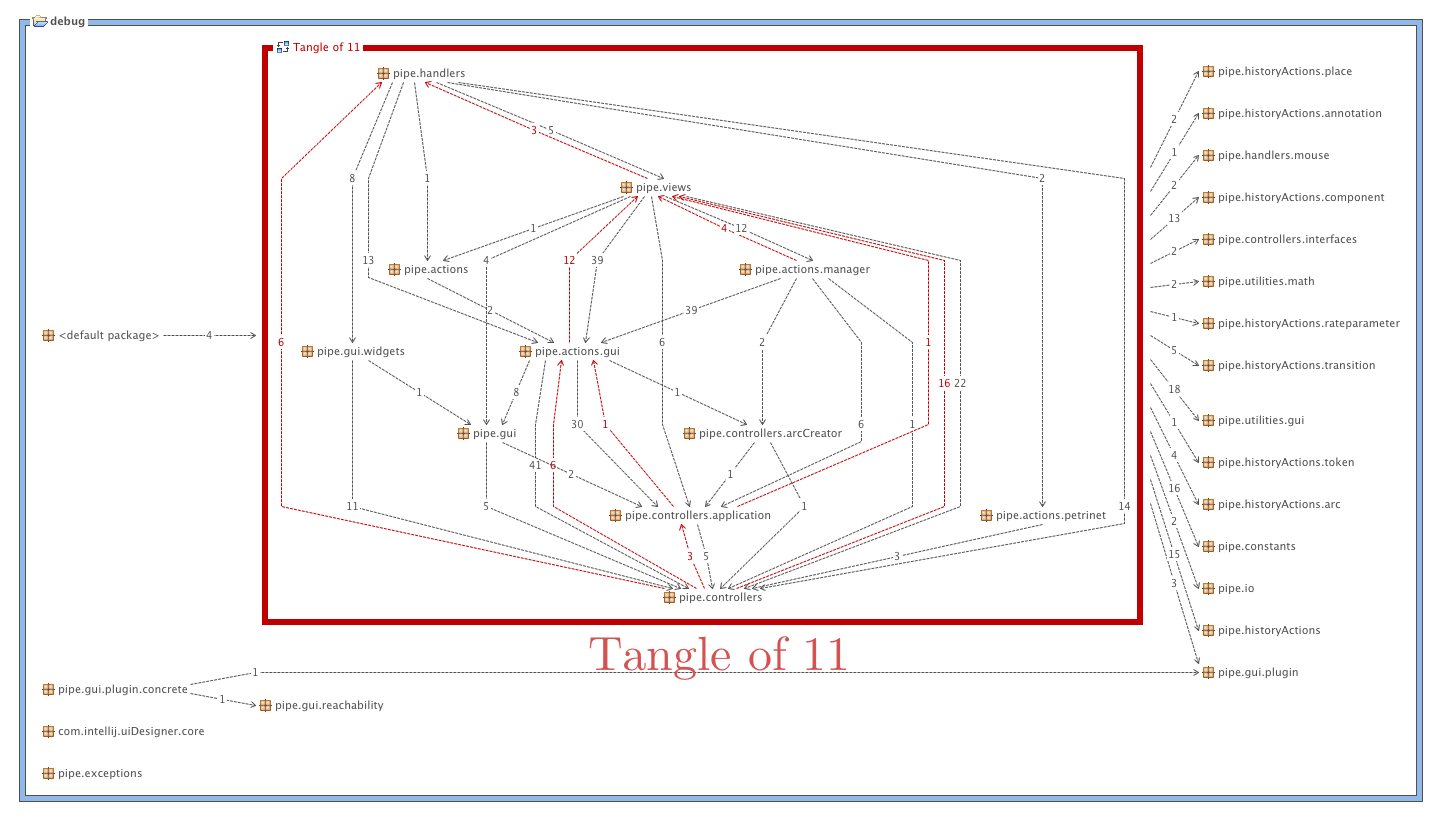
\includegraphics[width=0.85\textwidth]{eval/gui_tangle_annotated.png} 
}
% \caption{Tangle results}
\label{fig:tangle_results}
\end{center}
\end{figure}
\begin{figure}[tbp]
\begin{center}
\ContinuedFloat
\subcaptionbox{The new PIPE 5 tangle graph for the PIPECore repository reporting a single tangle of size 2. This tangle is between the functional expression parsers and the Petri net models. It has been kept because it improves the quality of the API by allowing Petri net components, namely transitions, to be able to evaluate their functional expressions without extra interaction from the user.}{
    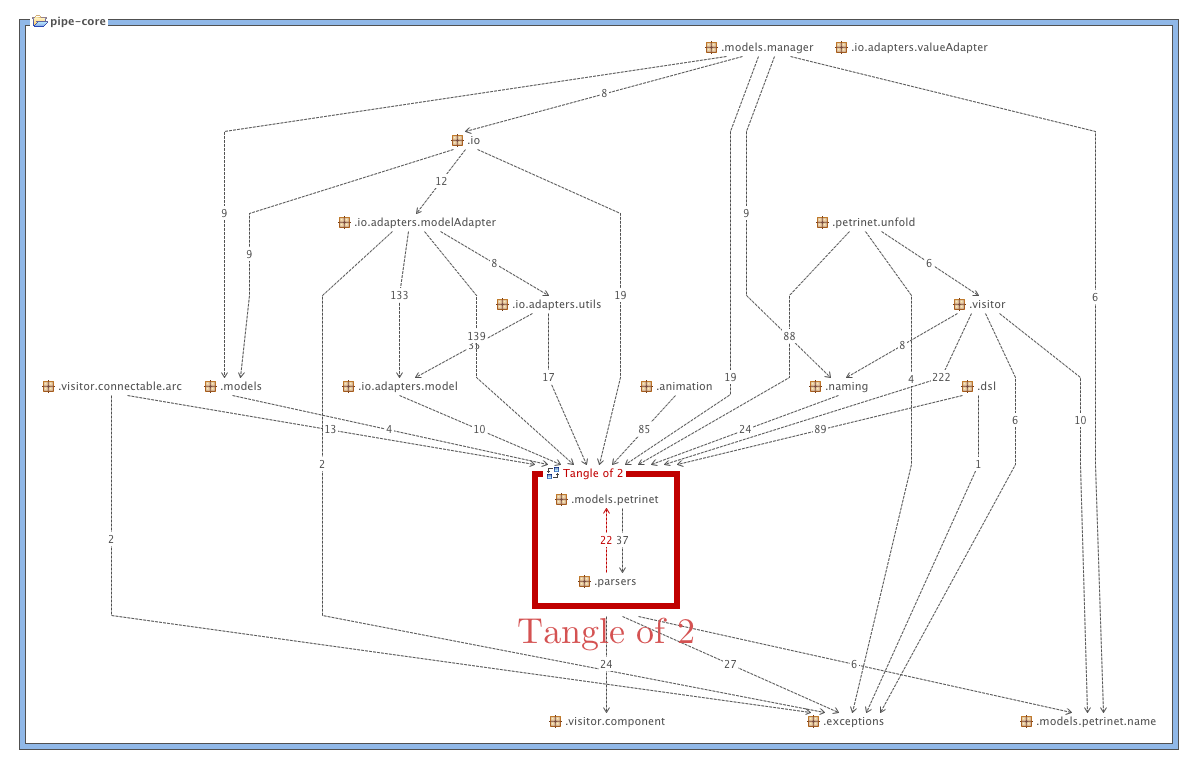
\includegraphics[width=0.85\textwidth]{eval/pipe_core_tangle_annotated.png} 
}
\subcaptionbox{The tangle graph for the new PIPEAnalysis repository containing the code for the steady state solver and the state space exploration. It reports 0 tangles.}{
    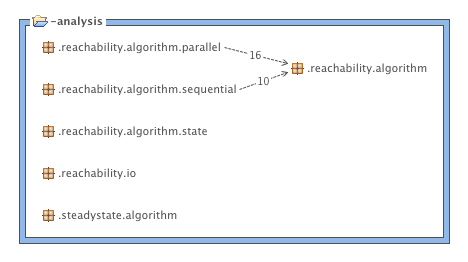
\includegraphics[scale=0.4]{eval/pipe_analysis_tangle.png} 
}
\hspace{5mm}
\subcaptionbox{The tangle graph for the new PIPEMarkovChain repository containing the classes which represent the underlying Markov chain of a Petri net and the explored sets data structure. It reports 0 tangles.}{
    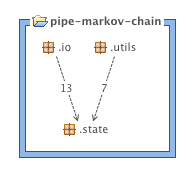
\includegraphics[scale=0.6]{eval/pipe_markov_chain_tangle.png} 
}
\caption{A comparison of the tangles in the PIPE 5 architecture against those in the PIPE 4 architecture. The tangle graphs clearly show a reduction from four tangles of size 18, 10, 7 and 5 down to only two tangles of size 11 and 2.}
\label{fig:tangle_results}
\end{center}
\end{figure}
\subsection{Static analysis}
By analysing the separate repositories we can see that the previous count of \num{12904} reported issues for PIPE 4 has been considerably reduced to a total of \num{937} issues. The break down of quality issues across repositories can be seen in \cref{tbl:pipe5_qaplug}.

\begin{table}[tb]
\small
\begin{center}
  \begin{tabular}{| l | c | c | c | c | c | c |}
    \hline
    Repository & Efficiency & Maintainability & Portability & Reliability & Usability & \textbf{Total} \\ 
    \hline
    PIPEMarkovChain & 0 & 0 & 0 & 0 & 0 & \textbf{0}\\ 
    \hline
    PIPEAnalysis & 0 & 0 & 0 & 0 & 0 & \textbf{0}\\    
    \hline
    PIPECore & 0 & 19 & 0 & 68 & 294 & \textbf{381}\\
    \hline
    PIPE & 13 & 77 & 0 & 426 & 40 & \textbf{556}\\
    \hline
    \textbf{Total} & \textbf{13} & \textbf{96} & \textbf{0} & \textbf{494} & \textbf{334} & {\color{red}\textbf{937}}\\
    \hline

  \end{tabular}
\caption{Break down of issues highlighted by the QAPlug analysis plug-in for Intellij for
each of the new PIPE 5 repositories. The total number of code quality issues for the entire project has been reduced from \num{12904} to \num{937}. Of these \num{937} issues \num{349} are due to auto-generated code via the ANTLR v4 plug-in.
On analysing these code quality issues we found that \num{349} of them are due to the ANTLR v4 auto-generated code meaning that the number of code quality issues for our written code is actually \num{588}. 
Of the remaining issues in the view codebase a total of \num{473} come from the \textit{`Magic Number Count'} metric. These are entirely due to layout and sizing settings for view components and indicate that whilst a useful metric for non-view code it is perhaps not so relevant for projects containing GUI code.
}
\label{tbl:pipe5_qaplug}
\end{center}
\end{table}

Furthermore Stan4J reported that the project size has reduced by a third from around \num{66000} lines of code to \num{22000} which is far more maintainable.



\subsection{Analysing the new modules}
Our new sequential state space exploration algorithm  yields increasing speedups compared to PIPE 4 for small state spaces as can be seen in \cref{tbl:pipe5_vs_pipe4_sequential}. Interestingly the algorithm for the sequential exploration does not differ from that of PIPE 4, the speedup comes from advanced data structure usage, memoization and other optimisation techniques.

\begin{table}[tb]
\begin{center}
  \begin{tabular}{| c | c | c | c | c | }
  \hline
    Number of states & Number of transitions & PIPE 4 (s) & PIPE 5 (s) & Speedup \\
    \hline
    40 & 156 & 0.21 & 0.17 & 1.24\\
    \hline
    100 & 480 & 0.36 & 0.40 & 0.90\\
    \hline
    625 & 4000 & 25.12 & 1.35 & 18.61\\
    \hline
    1350 & 9450 & 83.67 & 1.75 & 47.81\\
    \hline
    4096 & 28672 & 728.02 & 3.82 & 190.58\\
    \hline
    11664 & 93312 & 2738.37 & 8.51 & 321.78\\
    \hline
  \end{tabular}
\caption{The time taken in seconds to generate the reachability graph in PIPE 4 compared with the new sequential algorithm in PIPE 5. For very small state spaces we can see that the times are comparable, but for moderate sized Petri nets PIPE 5 is more scalable.}
\label{tbl:pipe5_vs_pipe4_sequential}
\end{center}
\end{table}

% Next we compare our sequential algorithm to our MapReduce-style parallel algorithm running on 4 virtual cores. Since the underlying algorithm performed  is very similar we expect to see a linear speedup and indeed the results in \cref{fig:parallel_vs_sequential_algo} show approximately this. We allowed each worker thread to process 100, 200, 500 states before returning to have their results reduced and although there is little difference between them, the 100 states per thread run provides the best speedup against the sequential implementation. Using these results we went on to investigate the benefits for larger state spaces and observed that we see similar speedups in \cref{fig:pipe5_large_state_space}.

% \begin{figure}[tb]
\internal{}
\setfigname{}
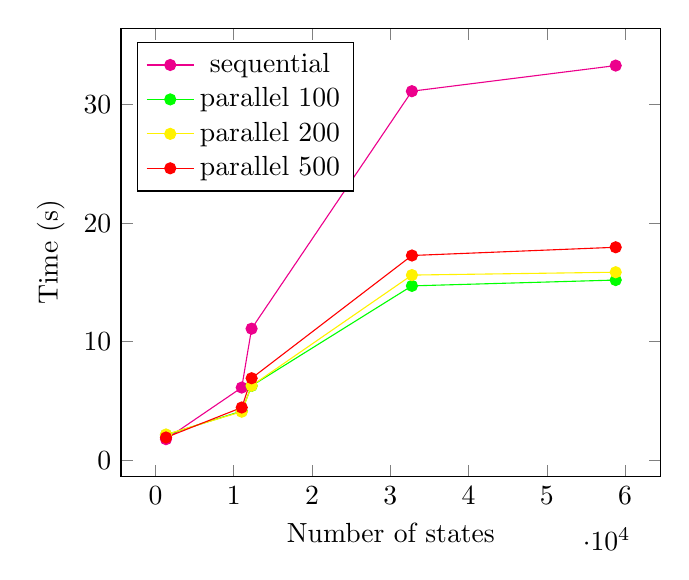
\begin{tikzpicture}
\definecolor{color0}{rgb}{0.75,0,0.75}

\begin{axis}[legend style={legend pos=north west},
ylabel={Time (s)},
xlabel={Number of states},
legend entries={{sequential},{parallel 100},{parallel 200},{parallel 500}}
% scaled ticks=false
]

% Sequential
\addplot [magenta, mark=*, mark size=2pt]
coordinates {
(1350,    1.783922000)
(11025,   6.135198000)
(12284,  11.098990000)
(32762,  31.121684000)
(58800,  33.280614000)
};

% 100
\addplot [green, mark=*, mark size=2pt]
coordinates {
(1350,   2.141683000)
(11025,  4.152756000)
(12288,  6.279725000)
(32768, 14.708286000)
(58800, 15.199168000)
};

% 200
\addplot [yellow, mark=*, mark size=2pt]
coordinates {
(1350,   2.177722000)
(11025,  4.099828000)
(12288,  6.293006000)
(32768, 15.619113000)
(58800, 15.858879000)
};

% 500
\addplot [red, mark=*, mark size=2pt]
coordinates {
(1350,   1.926380000)
(11025,  4.453230000)
(12288,  6.920561000)
(32768, 17.269375000)
(58800, 17.962744000)
};


\end{axis}
\end{tikzpicture}
\caption{A comparison between the run-times of PIPE 5's sequential state space exploration algorithm and the new MapReduce-style parallel algorithm running on 4 cores. We have allowed the parallel implementation to explore 500, 200, and 100 states before the reduction phase of each iteration. All parallel implementations yield at least a 2x speedup over the sequential algorithm although the 100 states per thread run performs slightly better than the others.}
\label{fig:parallel_vs_sequential_algo}
\end{figure}
% \begin{figure}[tb]
\internal{}
\setfigname{}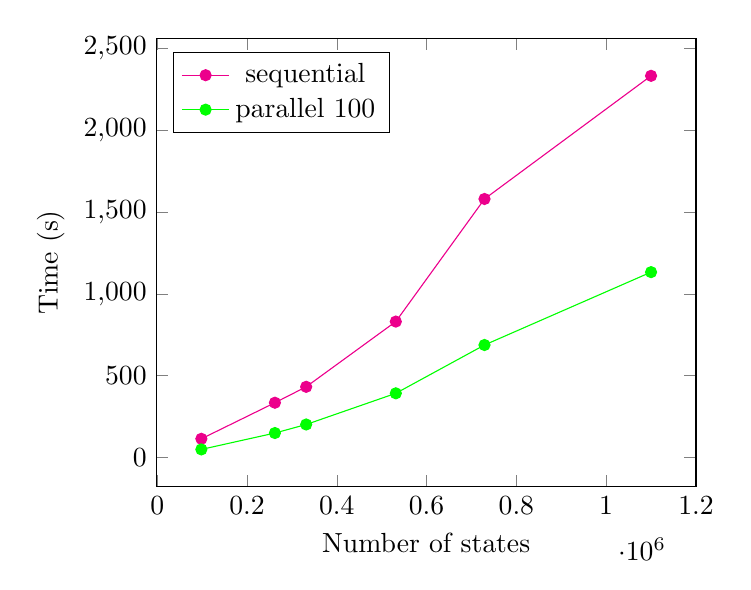
\begin{tikzpicture}
\definecolor{color0}{rgb}{0.75,0,0.75}

\begin{axis}[legend style={legend pos=north west},
ylabel={Time (s)},
xlabel={Number of states},
legend entries={{sequential},{parallel 100}}
% scaled ticks=false
]

% Sequential
\addplot [magenta, mark=*, mark size=2pt]
coordinates {
(98304,    113.690935000)
(262144,   334.272121000)
(331776,   431.582282000)
(531441,   830.441474000)
(729000,  1580.024665000)
(1099999, 2332.978991000)
};

% 100
\addplot [green, mark=*, mark size=2pt]
coordinates {
(98304,     48.798438000)
(262144,   148.977296000)
(331776,   201.183179000)
(531441,   391.800028000)
(729000,   687.234732000)
(1099999, 1132.697077000) % This is slightly over half an hr at 31 mins!
};

\end{axis}
\end{tikzpicture}
\caption{A comparison between the run-times of PIPE 5's sequential state space exploration algorithm and the new MapReduce-style parallel algorithm running on 4 cores for large Petri nets. This shows that the parallel implementation is consistently around twice as fast.}
\label{fig:pipe5_large_state_space}
\end{figure}

% Overall these results show a considerate speedup and allow for Petri nets with large state spaces to be analysed realistically on local machines.

To investigate the scalability of our parallel algorithm we analyse the new sequential and parallel algorithms against each other using a machine with a 3.40Ghz quad-core i7 processor. \cref{fig:scalability} shows that whilst the speedup from 2 to 4 virtual cores is promising at around 60\%, we do not get such good results from running the algorithm with 8 virtual cores. On profiling we found that the bottleneck in our algorithm is the creation of a states primary and secondary hash codes, taking 68\% of the algorithms run-time. Unfortunately since there is no implementation of a concurrent queue in Java that does not allow duplicates, we discovered that quite often it is possible to add a state twice to the exploration queue, meaning that its successors get generated twice too, causing their hash codes to be re-calculated.

\begin{figure}[ptb]
 \hspace*{\fill}%

\subcaptionbox{The raw times of the steady state exploration graph. The results gathered are for a sequential algorithm and for a parallel implementation with 100 states per thread running on 2, 4, and 8 virtual cores.} {
    \setfigname{}
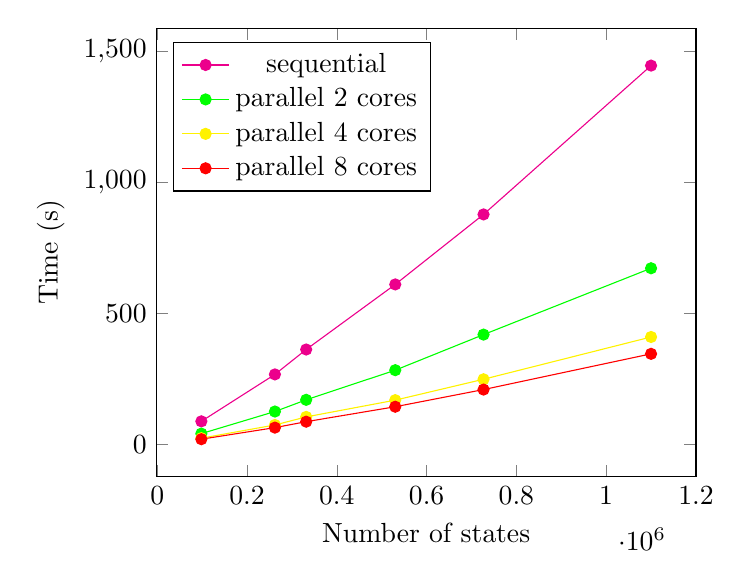
\begin{tikzpicture}
\definecolor{color0}{rgb}{0.75,0,0.75}

\begin{axis}[legend style={legend pos=north west},
ylabel={Time (s)},
xlabel={Number of states},
legend entries={{sequential},{parallel 2 cores},{parallel 4 cores},{parallel 8 cores}}
% scaled ticks=false
]

% Sequential
\addplot [magenta, mark=*, mark size=2pt]
coordinates {
(98279,     88.633369210) 
(262144,   267.658476596) 
(331776,   362.664597933) 
(530202,   610.926546563) 
(726836,   878.042343995) 
(1099999, 1445.821632163) 
};

% 2
\addplot [green, mark=*, mark size=2pt]
coordinates {
(98279,    41.786394435)
(262144,  126.064339906)
(331776,  170.664153825)
(530202,  283.808419361)
(726836,  419.506128369)
(1099999, 672.649284048)
};

% 4
\addplot [yellow, mark=*, mark size=2pt]
coordinates {
(98279,    24.373880968) 
(262144,   74.762257833) 
(331776,  105.559247500)
(530202,  169.459170682)
(726836,  249.133023117)
(1099999, 410.412285810)
};

% 8
\addplot [red, mark=*, mark size=2pt]
coordinates {
(98279,    20.521322935)  
(262144,   64.652309353)  
(331776,   87.323938113) 
(530202,  144.356493902) 
(726836,  209.819065630) 
(1099999, 346.097981548) 
};


\end{axis}
\end{tikzpicture}

}\hfill
\subcaptionbox{The relevant speedup gained over the sequential algorithm running our parallel algorithm with 100 states per thread and an increasing number of virtual cores. The graph shows that for each increase in the number of virtual cores we see a consistent speedup.} {
    \setfigname{}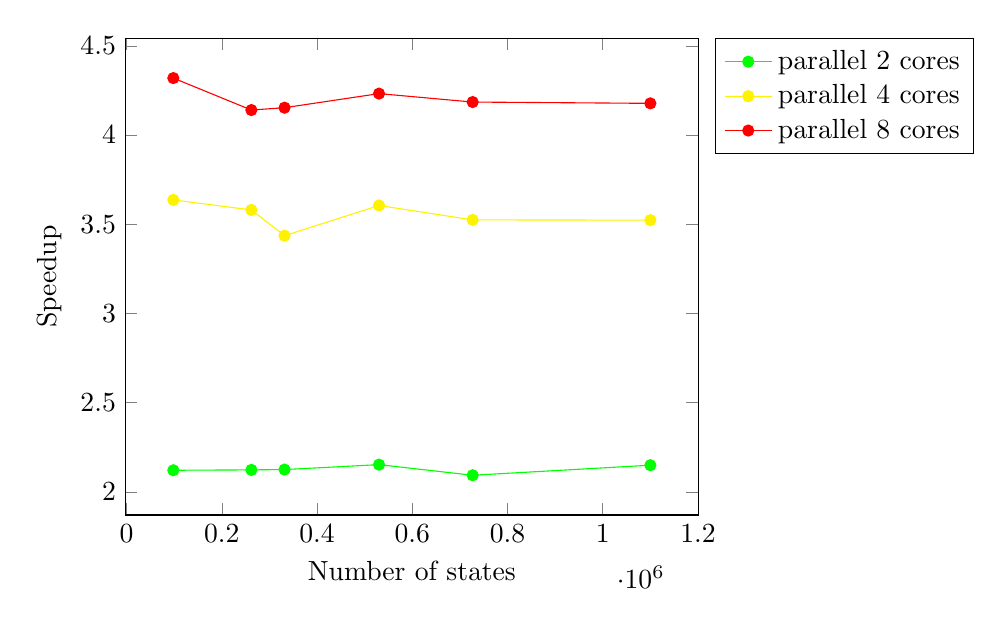
\begin{tikzpicture}
\definecolor{color0}{rgb}{0.75,0,0.75}

\begin{axis}[width=0.73\textwidth,
legend style={legend pos=outer north east},
ylabel={Speedup},
xlabel={Number of states},
legend entries={{parallel 2 cores},{parallel 4 cores},{parallel 8 cores}}
% scaled ticks=false
]

% 2
\addplot [green, mark=*, mark size=2pt]
coordinates {
(98279,   2.1211059343220406) % 99860326918 / 51611435904
(262144,  2.1231894506851012) % 304887660912 / 158793100442 
(331776,  2.1250191666193614) % 407267170985 / 208514610650
(530202,  2.152601913426362) % 709773626643 / 362338733157
(726836,  2.093038181369949) % 1023339231997 / 523542258224
(1099999, 2.149443501169068) % 1621045044327 / 845268409674
};

% 4
\addplot [yellow, mark=*, mark size=2pt]
coordinates {
(98279,   3.6364077319637786) % 99860326918 / 30575984607
(262144,  3.5801283208150485) % 304887660912 / 93863598681
(331776,  3.43564970878558) % 407267170985 / 127750195215
(530202,  3.605154823455611) % 709773626643 / 215606239138
(726836,  3.5243916402950974) % 1023339231997 / 318285464137
(1099999, 3.522851732641215) % 1621045044327 / 515475748470
};

% 8
\addplot [red, mark=*, mark size=2pt]
coordinates {
(98279,   4.319086517508672) % 99860326918 / 26825872545
(262144,  4.139967764099366) % 304887660912 / 82619391439
(331776,  4.153094853139814) % 407267170985 / 110556083237
(530202,  4.232068333397891) % 709773626643 / 189352805147
(726836,  4.184759575392262) % 1023339231997 / 282687963976
(1099999, 4.177492239903399) % 1621045044327 / 456685753436
};


\end{axis}
\end{tikzpicture}

}
\hspace*{\fill}%
\caption{A comparison between the run-times and relevant speedup of PIPE 5's sequential state space exploration and its parallel algorithm with 100 states per thread running on 2, 4 and 8 virtual cores on a 3.2GHz quad-core hyper-threaded 3rd generation i7 processor.}
\label{fig:scalability}
\end{figure}

Nevertheless in order to put into perspective the speedup gained by our new parallel algorithm using 100 states per thread and 8 virtual-cores we compared the run-times of a 4096 state Petri net with this algorithm and PIPE 4. Whilst PIPE 4 explores the state space in 9.37 minutes, our new algorithm can explore it in 2.65 seconds which amounts to an incredible 211x speedup. Moreover our new algorithm can solve a Petri net with \num{1099999} states in 5.77 minutes which is faster than the time taken to solve the 4096 state Petri net in PIPE 4!


\subsection{Testimonial}
The following testimonial from Steve Doubleday a researcher at University of California Irvine, who works closely with the International Computer Science Institute (ICSI), summaries the key architectural achievements of this project:

\begin{quote}
\singlespacing
    \textit{``PIPE has been re-engineered top to bottom, as part of its most significant upgrade in years. Key improvements are the separation of business logic from the GUI, the addition of a large suite of unit tests, and the re-packaging of the software as Maven artifacts.  All of this makes my work significantly easier. The work at ICSI (International Computer Science Institute), and my own dissertation both rely on extensions to the basic PetriNet capabilities, to better enable the creation of neurally-plausible cognitive models of action. The existing ICSI software consists of many modifications to a very old version of PIPE. My intent is to re-build the existing ICSI software on top of the new PIPE artifacts. This will make both current development and future maintenance much cleaner, and will also make it more attractive to other cognitive scientists to re-use the ICSI extensions.''}
\end{quote}
